\documentclass{article}
\usepackage[dvipsnames]{xcolor}
\usepackage[margin=1in]{geometry}
\usepackage{amsmath, amssymb, amsthm}
\usepackage{enumitem}

%Creating Figures
\usepackage{subcaption}

%Creating Figures
\usepackage{tikz}
\usetikzlibrary{calc,spy}

%Extra Math
\usepackage{mathtools}

%Formatting and Spacing
\setitemize[1]{noitemsep, parsep = 5pt, topsep = 5pt}
\setenumerate[1]{label = (\alph*), parsep = 1pt, topsep = 5pt}
\setlength\parindent{0pt}
\linespread{1.1}

%Easy Numbering
\newcounter{counter}
\newcommand{\Exercise}{Exercise \stepcounter{counter}\thecounter}

%Cases Environment
\newlist{Cases}{enumerate}{3}
\setlist[Cases]{leftmargin = .25in, label = {Case \arabic*.}, topsep = 0.01in, itemsep = 0.04in, itemindent = .5in, parsep = 0in}

%Custom Title Fields
\newcommand{\hmwkTitle}{Homework 4 (with Solutions)}
\newcommand{\hmwkDueDate}{Feb 19, 2022}
\newcommand{\hmwkClass}{Honors Discrete Mathematics}
\newcommand{\hmwkClassInstructor}{Professor Gerandy Brito}
\newcommand{\hmwkSection}{Spring 2022}
\newcommand{\hmwkAuthorName}{Sarthak Mohanty}

%Headers and Footers
\usepackage{fancyhdr}
\usepackage{extramarks}
\pagestyle{fancy}
\lhead{\hmwkAuthorName}
\chead{\hmwkClass \ (\hmwkClassInstructor)}
\rhead{Homework 4}
\cfoot{\thepage}
\renewcommand\headrulewidth{0.4pt}
\renewcommand\footrulewidth{0.4pt}

\title{
    \vspace{2in}
    \textbf{\hmwkClass:\\ \hmwkTitle}\\
    \normalsize\vspace{0.1in}\small{Due\ on\ \hmwkDueDate\ at 11:59pm}\\
    \vspace{0.1in}\large{\textit{\hmwkClassInstructor\ \hmwkSection}}
    \vspace{3in}
    \author{\textbf{\hmwkAuthorName}}
    \date{}
}

\begin{document}

\maketitle
\pagebreak

\subsection*{\Exercise}
    Prove that for each $x \in \mathbb{Z}$, 6 divides $x^3 - x$.
    
    \vspace{1.5mm}
    {\small \textit{Hint}: Use induction to prove the statement for any $x \in \mathbb{N}$, then extend this reasoning to all $x \in \mathbb{Z}$.}

%Note for next semester: Make sure that they prove by induction next time.

\subsection*{Solution}
    Let $P(x)$ be the sentence $$6 \mid x^3 - x.$$
    \textsc{Part 1.} First, we shall prove by induction that for each $x \in \mathbb{N}$, $P(x)$ is true.
    \begin{enumerate} [label = {}, nosep, leftmargin = .25in]
        \item \textsc{Base Case}: $P(0)$ is true, since $0^3 - 0 = 0$ and $0 \mid 6$.
        \item \textsc{Inductive Step}: Now let $x \in \mathbb{N}$ such that $P(x)$ is true. Then 
        $$(x + 1)^3 - (x + 1) = x^3 + 3x^2 + 2x = (x^3 - x) + 3x(x + 1).$$
        Looking at the $3x(x + 1)$ term, since $x$ or $x + 1$ must be even, $x(x + 1)$ must be even as well. This means that $2 \mid x(x + 1)$ and $6 \mid 3x(x + 1)$. From our initial assumption, we know that $6 \mid x^3 - x$. Since $6 \mid x^3 - x$ and $6 \mid x(x + 1)$, we know that $6 \mid (x^3 - x) + 3x(x + 1)$. Hence $P(x + 1)$ is true as well.
        \item \textsc{Conclusion}: Therefore by induction, for all $x \in \mathbb{N}$, $P(x)$ is true.
    \end{enumerate}
    
    \vspace{1.5mm}
    \textsc{Part 2.} Now consider any $x \in \mathbb{Z}$. Then $x \ge 0$ or $x \le -1$. 
    
    \begin{Cases}
        \item Suppose $x \ge 0$. Then $x \in \mathbb{N}$, so $P(x)$ is true by part 1. 
        \item Suppose $x \le -1$. Then $-x \in \mathbb{N}$, so $P(-x)$ is true, or equivalently, $6 \mid (-x)^3 - (-x)$. Then there exists an integer $k$ such that $(-x)^3 - (-x) = 6k$. Rearranging, we get $x^3 - x = 6(-k)$. Therefore $6 \mid x^3 - x$. In other words, $P(x)$ is true.
    \end{Cases}
    In either case, $P(x)$ is true. Hence for all $n \in \mathbb{N}$, $P(n)$ is true.

\subsection*{\Exercise}
    Landscaper Larry is planning on remodeling a square enclosure. He wants to split it up into multiple smaller square enclosures. However, he does not know how many enclosures he will need to make. Prove using induction that Larry can divide any square enclosure into $n$ smaller square enclosures for $n \ge 6$. Include drawing(s) of your work.

\subsection*{Solution}
    Let $P(n)$ be the sentence $$\text{Any square can be split into $n$ smaller squares.}$$
    \textsc{Base Case}: We can split any square into $6$, $7$, and $8$ smaller squares, as shown in Figure \ref{fig:Q3 Base Case}. Hence $P(6)$, $P(7)$, and $P(8)$ are all true. \\
    \textsc{Inductive Step}: Now let $n \ge 6$ such that $P(n), P(n + 1), P(n + 2)$ is true. Consider the splitting of a square into $n$ smaller squares. Choose one of these smaller squares, and split it into four squares of even smaller size, as shown in Figure \ref{fig:Q3 Inductive Step}. This gives a splitting of $n + 3$ squares. Hence $P(n + 3)$ is true as well. \\
    \textsc{Conclusion}: Therefore by strong induction, for all $n \ge 6$, $P(n)$ is true.
    
    \pgfmathsetmacro{\relativefibrethickness}{0.50}
    \pgfmathsetmacro{\relativefibrevariation}{0.07}
    \pgfmathsetmacro{\numberoffibres}{15}
    \pgfmathsetmacro{\fibresteps}{50}
    \pgfmathsetmacro{\boardwidth}{3}
    \pgfmathsetmacro{\boardheight}{3}
    \newcommand{\backgroundcolor}{ForestGreen}
    \newcommand{\fibrecolor}{ForestGreen!90!black}
    
    \begin{figure}[htbp]
         \centering
        \begin{subfigure}{0.3\textwidth}
            \centering
            \begin{tikzpicture}[scale = 0.67, spy using outlines={circle, size=3cm, connect spies}]
                 \pgfmathsetmacro{\segmentwidth}{\boardwidth/(\numberoffibres+1)}
                \pgfmathsetmacro{\segmentvariation}{\relativefibrethickness/2*\segmentwidth}
            
                \pgfmathsetmacro{\secondfibre}{2*\segmentwidth}
                \pgfmathsetmacro{\lastfibre}{\numberoffibres*\segmentwidth}
            
                \pgfmathsetmacro{\stepheight}{\boardheight/\fibresteps}
            
                %auto generated courtyard
                \filldraw[\backgroundcolor] (0,0) rectangle (\boardwidth,\boardheight);
                
                \foreach \x in {1,2,...,\numberoffibres}
                {   \fill[\fibrecolor] ($(\x*\segmentwidth-\segmentvariation,0) + (rand*\relativefibrevariation*\relativefibrethickness,0)$) 
                    \foreach \y in {1,...,\fibresteps}
                    {   -- ($(\x*\segmentwidth-\segmentvariation,\y*\stepheight) + (rand*\relativefibrevariation*\relativefibrethickness,0)$)
                    }
                    -- ($(\x*\segmentwidth+\segmentvariation,\boardheight)+ (rand*\relativefibrevariation*\relativefibrethickness,0)$) 
                    \foreach \y in {\fibresteps,...,0}
                    {   -- ($(\x*\segmentwidth+\segmentvariation,\y*\stepheight) + (rand*\relativefibrevariation*\relativefibrethickness,0)$)
                    }
                    -- cycle;
                }
                \draw[thick] (0,0) rectangle (\boardwidth,\boardheight);
            
                % manually added squares
                \draw (0,0) grid (1,3);
                \draw (1,2) grid (3,3);
                % spy for seeing the structure
                % \spy[magnification=3,blue] on (1,1) in node at (15,5);
            \end{tikzpicture}
            \caption{$n = 6$}
        \end{subfigure}
        \pgfmathsetmacro{\boardwidth}{4}
        \pgfmathsetmacro{\boardheight}{4}
        \begin{subfigure}{0.3\textwidth}
            \centering
            
            \pgfmathsetmacro{\segmentwidth}{\boardwidth/(\numberoffibres+1)}
            \pgfmathsetmacro{\segmentvariation}{\relativefibrethickness/2*\segmentwidth}
        
            \pgfmathsetmacro{\secondfibre}{2*\segmentwidth}
            \pgfmathsetmacro{\lastfibre}{\numberoffibres*\segmentwidth}
        
            \pgfmathsetmacro{\stepheight}{\boardheight/\fibresteps}
            \begin{tikzpicture}[scale = 0.5, spy using outlines={circle, size=3cm, connect spies}]
                %auto generated courtyard
                \filldraw[\backgroundcolor] (0,0) rectangle (\boardwidth,\boardheight);
                
                \foreach \x in {1,2,...,\numberoffibres}
                {   \fill[\fibrecolor] ($(\x*\segmentwidth-\segmentvariation,0) + (rand*\relativefibrevariation*\relativefibrethickness,0)$) 
                    \foreach \y in {1,...,\fibresteps}
                    {   -- ($(\x*\segmentwidth-\segmentvariation,\y*\stepheight) + (rand*\relativefibrevariation*\relativefibrethickness,0)$)
                    }
                    -- ($(\x*\segmentwidth+\segmentvariation,\boardheight)+ (rand*\relativefibrevariation*\relativefibrethickness,0)$) 
                    \foreach \y in {\fibresteps,...,0}
                    {   -- ($(\x*\segmentwidth+\segmentvariation,\y*\stepheight) + (rand*\relativefibrevariation*\relativefibrethickness,0)$)
                    }
                    -- cycle;
                }
                \draw[thick] (0,0) rectangle (\boardwidth,\boardheight);
            
                % manually added squares
                \draw (0,2) grid (2,4);
                \draw[step = 2] (0,0) grid (4,4);
            \end{tikzpicture}
        \caption{$n = 7$}
        \end{subfigure}
        \begin{subfigure}{0.3\textwidth}
            \centering
            
            \pgfmathsetmacro{\segmentwidth}{\boardwidth/(\numberoffibres+1)}
            \pgfmathsetmacro{\segmentvariation}{\relativefibrethickness/2*\segmentwidth}
        
            \pgfmathsetmacro{\secondfibre}{2*\segmentwidth}
            \pgfmathsetmacro{\lastfibre}{\numberoffibres*\segmentwidth}
        
            \pgfmathsetmacro{\stepheight}{\boardheight/\fibresteps}
            \begin{tikzpicture}[scale = 0.5, spy using outlines={circle, size=3cm, connect spies}]
                %auto generated courtyard
                \filldraw[\backgroundcolor] (0,0) rectangle (\boardwidth,\boardheight);
                
                \foreach \x in {1,2,...,\numberoffibres}
                {   \fill[\fibrecolor] ($(\x*\segmentwidth-\segmentvariation,0) + (rand*\relativefibrevariation*\relativefibrethickness,0)$) 
                    \foreach \y in {1,...,\fibresteps}
                    {   -- ($(\x*\segmentwidth-\segmentvariation,\y*\stepheight) + (rand*\relativefibrevariation*\relativefibrethickness,0)$)
                    }
                    -- ($(\x*\segmentwidth+\segmentvariation,\boardheight)+ (rand*\relativefibrevariation*\relativefibrethickness,0)$) 
                    \foreach \y in {\fibresteps,...,0}
                    {   -- ($(\x*\segmentwidth+\segmentvariation,\y*\stepheight) + (rand*\relativefibrevariation*\relativefibrethickness,0)$)
                    }
                    -- cycle;
                }
                \draw[thick] (0,0) rectangle (\boardwidth,\boardheight);
            
                % manually added squares
                \draw (0,0) grid (1,4);
                \draw (0,3) grid (4,4);
            \end{tikzpicture}
        \caption{$n = 8$}
        \end{subfigure}
        \caption{Base Cases for Question 3}
        \label{fig:Q3 Base Case}
    \end{figure}
    
    
    \begin{figure}[htbp]
        \centering
        \hspace{3cm}
        \begin{tikzpicture}[scale = 0.67, spy using outlines={circle, size=2cm, connect spies}]
             \pgfmathsetmacro{\segmentwidth}{\boardwidth/(\numberoffibres+1)}
            \pgfmathsetmacro{\segmentvariation}{\relativefibrethickness/2*\segmentwidth}
        
            \pgfmathsetmacro{\secondfibre}{2*\segmentwidth}
            \pgfmathsetmacro{\lastfibre}{\numberoffibres*\segmentwidth}
        
            \pgfmathsetmacro{\stepheight}{\boardheight/\fibresteps}
        
            %auto generated courtyard
            \filldraw[\backgroundcolor] (0,0) rectangle (\boardwidth,\boardheight);
            
            \foreach \x in {1,2,...,\numberoffibres}
            {   \fill[\fibrecolor] ($(\x*\segmentwidth-\segmentvariation,0) + (rand*\relativefibrevariation*\relativefibrethickness,0)$) 
                \foreach \y in {1,...,\fibresteps}
                {   -- ($(\x*\segmentwidth-\segmentvariation,\y*\stepheight) + (rand*\relativefibrevariation*\relativefibrethickness,0)$)
                }
                -- ($(\x*\segmentwidth+\segmentvariation,\boardheight)+ (rand*\relativefibrevariation*\relativefibrethickness,0)$) 
                \foreach \y in {\fibresteps,...,0}
                {   -- ($(\x*\segmentwidth+\segmentvariation,\y*\stepheight) + (rand*\relativefibrevariation*\relativefibrethickness,0)$)
                }
                -- cycle;
            }
            \draw[thick] (0,0) rectangle (\boardwidth,\boardheight);
        
            % manually added squares
            \draw (0,0) grid (3,3);
            \draw[densely dashed, step = 0.5] (2,0) grid (3,1);
            % spy for seeing the structure
            \spy[magnification=2, brown] on (1.67,0.3) in node at (6, 1.5);
        \end{tikzpicture}
        \caption{A demonstration of the inductive step. Here we show $P(9) \implies P(12)$.}
        \label{fig:Q3 Inductive Step}
    \end{figure}

\subsection*{\Exercise}
    Suppose now we have an infinite chessboard, with each square labeled as coordinates $(i, j)$ with $i, j \in \mathbb{N}$. A knight starts at the square $(0, 0)$ (in other words, it has already visited this square). Use induction to prove that this knight can visit every square using a finite sequence of moves.
    
    {\small \vspace{1.5mm} 
    Hint: Use induction on the variable $n = i + j$.}
    
\subsection*{Solution}
    Let $P(n)$ be the statement $$\text{A knight can visit all squares $(i, j)$, where $i + j \le n$}$$
    \textsc{Base Case}: $P(2)$ is true, as the knight can visit all $6$ squares $(i, j)$, where $i + j \le 2$. The paths for each point are shown below, with corresponding illustrations in Figure \ref{fig:Q4 Base Case}.
    
    \begin{itemize}[label = {}]
        \item $(0, 0)$: The knight has already reached this point
        \item $(0, 1)$: The knight moves from $(0, 0)$ to $(1, 2)$ to $(2, 0)$ to $(0, 1)$.
        \item $(0, 2)$: The knight moves from $(0, 0$ to $(2, 1)$ to $(0, 2)$.
        \item $(1, 0)$: The knight moves from $(0, 0$ to $(2, 1)$ to $(0, 2)$ to $(1, 2)$
        \item $(1, 1)$: The knight moves from $(0, 0)$ to $(1, 2)$ to $(0, 1)$ to $(2, 2)$ to $(0, 3)$ to $(1, 1)$.
        \item $(2, 0)$: The knight moves from $(0, 0)$ to $(1, 2)$ to $(2, 0)$
    \end{itemize}
    \textsc{Inductive Step}: Now let $n \in \mathbb{N}$ such that $P(n)$ is true. We want to show $P(n + 1)$ is true; in other words, we wish to show that a knight can visit all squares $(i', j')$, where $i' + j' \le n + 1$.
    
    \vspace{1.5mm}
    Since $n + 1 \ge 3$, we can assume one of $i, j \ge 2$. Now $i' + j' -1 = n < n + 1$, so by the inductive hypothesis, the knight can visit any square of the form $(i' + 1, j' - 2)$. From there, it is just one move to the required square $(i', j')$. \\
    \textsc{Conclusion}: Therefore by induction, for all $n \ge 2$, $P(n)$ is true.
    
    \begin{figure}[htbp]
        \centering
        \begin{subfigure}{0.18\textwidth}
            \centering
            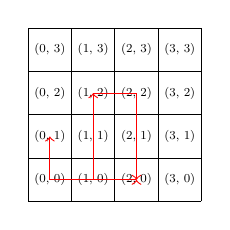
\begin{tikzpicture} [scale = 0.55, transform shape]
                \draw (0,0) grid (4, 4);
                \foreach \x in {0.5, 1.5, 2.5, 3.5}
                  \foreach \y in {0.5, 1.5, 2.5, 3.5}
                    \pgfmathsetmacro{\asd}{int(\x-0.5)}
                    \pgfmathsetmacro{\dsa}{int(\y-0.5)}
                    \node at (\x,\y) {\footnotesize (\asd, \dsa)};
                \draw [red, ->, to path={-| (\tikztotarget)}, yshift = 0.5cm, xshift = 0.5cm] (0,0) edge (1,2) (1,2) edge (2,0) (2,0) edge (0,1);
            \end{tikzpicture}
            \subcaption{(0,1)}
        \end{subfigure}
        \begin{subfigure}{0.18\textwidth}
            \centering
            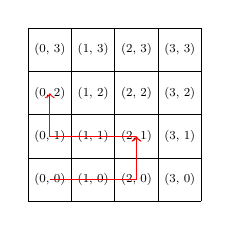
\begin{tikzpicture}[scale = 0.55, transform shape]
                \draw (0,0) grid (4, 4);
                \foreach \x in {0.5, 1.5, 2.5, 3.5}
                  \foreach \y in {0.5, 1.5, 2.5, 3.5}
                    \pgfmathsetmacro{\asd}{int(\x-0.5)}
                    \pgfmathsetmacro{\dsa}{int(\y-0.5)}
                    \node at (\x,\y) {\footnotesize (\asd, \dsa)};
                \draw [red, ->, to path={-| (\tikztotarget)}, yshift = 0.5cm, xshift = 0.5cm] (0,0) edge (2,1) (2,1) edge (0,2);
            \end{tikzpicture}
            \subcaption{(0,2)}
        \end{subfigure}
        \begin{subfigure}{0.18\textwidth}
            \centering
            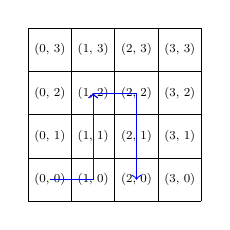
\begin{tikzpicture} [scale = 0.55, transform shape]
                \draw (0,0) grid (4, 4);
                \foreach \x in {0.5, 1.5, 2.5, 3.5}
                  \foreach \y in {0.5, 1.5, 2.5, 3.5}
                    \pgfmathsetmacro{\asd}{int(\x-0.5)}
                    \pgfmathsetmacro{\dsa}{int(\y-0.5)}
                    \node at (\x,\y) {\footnotesize (\asd, \dsa)};
                \draw [blue, ->, to path={-| (\tikztotarget)}, yshift = 0.5cm, xshift = 0.5cm] (0,0) edge (1,2) (1,2) edge (2,0);
            \end{tikzpicture}
            \subcaption{(1,0)}
        \end{subfigure}
        \begin{subfigure}{0.18\textwidth}
            \centering
            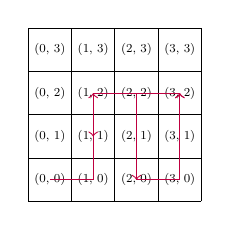
\begin{tikzpicture} [scale = 0.55, transform shape]
                \draw (0,0) grid (4, 4);
                \foreach \x in {0.5, 1.5, 2.5, 3.5}
                  \foreach \y in {0.5, 1.5, 2.5, 3.5}
                    \pgfmathsetmacro{\asd}{int(\x-0.5)}
                    \pgfmathsetmacro{\dsa}{int(\y-0.5)}
                    \node at (\x,\y) {\footnotesize (\asd, \dsa)};
                \draw [purple, ->, to path={-| (\tikztotarget)}, yshift = 0.5cm, xshift = 0.5cm] (0,0) edge (1,2) (1,2) edge (2,0) (2,0) edge (3,2) (3,2) edge (1,1);
            \end{tikzpicture}
            \subcaption{(1,1)}
        \end{subfigure}
        \begin{subfigure}{0.18\textwidth}
            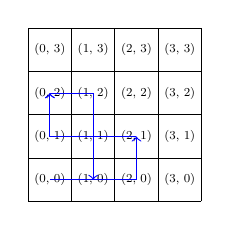
\begin{tikzpicture} [scale = 0.55, transform shape]
                \draw (0,0) grid (4, 4);
                \foreach \x in {0.5, 1.5, 2.5, 3.5}
                  \foreach \y in {0.5, 1.5, 2.5, 3.5}
                    \pgfmathsetmacro{\asd}{int(\x-0.5)}
                    \pgfmathsetmacro{\dsa}{int(\y-0.5)}
                    \node at (\x,\y) {\footnotesize (\asd, \dsa)};
                \draw [blue, ->, to path={-| (\tikztotarget)}, yshift = 0.5cm, xshift = 0.5cm] (0,0) edge (2,1) (2,1) edge (0,2) (0,2) edge (1,0);
            \end{tikzpicture}
            \subcaption{(2,0)}
        \end{subfigure}
        \caption{Base Cases for Question 4}
        \label{fig:Q4 Base Case}
    \end{figure}

\subsection*{\Exercise}
    The fabled city of Ba Sing Se has $2$ cats for every person, $2$ serpents for every bison, and $2$ lemurs for every cat. What is the greatest total number of people, bison, lemurs, serpents, and cats that \underline{cannot} exist in Ba Sing Se? Prove using induction.
    
    \vspace{1.5mm}
    {\small \textit{Hint}: We covered a problem in lecture that Professor Brito called the ``Bill Denomination" problem. Can you find some similarities?}

\subsection*{Solution}
    Let the number of cats be $c$, people be $p$, serpents be $s$, bison be $b$, and lemurs be $\ell$. We know
    \begin{align*}
        c &= 2p \\
        s &= 2b \\
        \ell &= 2c.
    \end{align*}
    Thus the total number of cats, people, serpents, bison, and lemurs is $$c + p + s + b + \ell = 2p + p + 2b + b + 2(2)p = 7p + 3b.$$ From here, this question becomes similar to one we did in lecture. \\
    Let $P(n)$ be the sentence $$\text{There can exist at least $n$ total number of animals and people in Ba Sing Se}.$$
    \textsc{Base Case}: 
    $$\begin{aligned}[t]
        \text{$P(12)$ is true, let $p = 0$ and $b = 4$.} \\
        \text{$P(13)$ is true, let $p = 1$ and $b = 2$.} \\
        \text{$P(14)$ is true, let $p = 2$ and $b = 0$.}
    \end{aligned}$$
    \textsc{Inductive Step}: Now let $n \ge 12$ such that $P(n)$, $P(n + 1)$, and $P(n + 2)$ are all true. Then by incrementing $b$ by one, $P(n + 3)$ is true as well. \\
    \textsc{Conclusion}: Therefore by strong induction, for all $n \ge 12$, $P(n)$ is true. 
    
    \vspace{3mm} Hence the greatest total number of people, bison, lemurs, goats, and cats that cannot exist in Ba Sing Se is equal to $12 - 1 = \boxed{11}$.

\subsection*{\Exercise}
    One day, you encounter a rather large farm. The very wise farmer informs you that there are exactly $2025$ cows in the farm. However, these cows have very poor memory. In order to make sure the cows remember each other, the farmer trained them until the following rule was satisfied: $$\text{Among each group of $4$ cows, there is at least one cow who knows each of the other three.}$$ The farmer explains that this rule ensures at least $2022$ cows know every other cow. You seem suspicious, and decide to prove the farmer's claim either correct or incorrect. Show this proof below. Is the farmer correct?
    
    \vspace{1.5mm}
    {\small \textit{Hint}: Sometimes we cannot use induction to prove a result, but we can use induction to prove a stronger result (in the textbook, this is called \textit{inductive loading}). Can you use induction to prove the farmer's claim for any $n$ cows on a farm?}
    
    %Note for next semester: $A$ knows $B$ was not specified to be symmetric. Either specify one, or make them prove it for both using induction.

\subsection*{Solution 1 (with Assumption)}
    \textit{Note: In this solution, the assumption was made that if cow $A$ knows cow $B$, then cow $B$ knows cow $A$.}

    \vspace{1.5mm}
    Let $P(n)$ be the sentence $$\text{In a farm with $n$ cows, there must be at least $n - 3$ cows who know every other cow.}$$

    \textsc{Base Case}: $P(4)$ is true by definition. \\
    \textsc{Inductive Step}:
    Let $n \ge 4$ such that $P(n)$ is true. We wish to prove $P(n + 1)$ is true. To do this, consider a farm with $n + 1$ cows. Choose $n$ cows (leaving one cow, $A$, out) and apply the inductive step to conclude that at least $(n - 3)$ cows know every other cow in the $n$-cow group, $G$.
    
    \begin{Cases}
        \item Suppose every cow in the group $G$ knows each other. Then take $3$ of these cows and $A$ to deduce that $A$ knows a cow $B \in G$, which means $B$ knows every other cow. Then apply the inductive step on the remaining $n$ cows (excluding $B$) to find $(n - 3)$ cows out of them that know every other cow (including $B$). Then these $(n - 3)$ cows and $B$, which enumerate $(n - 2)$ cows, know every other cow.
        \item Suppose there is exactly one cow in the group $G$ who does not know every other cow. This is impossible, so we disregard this case.
        \item Suppose there are exactly two cows $B, C \in G$ who do not know every other cow. Then the only possibility is that they do not know each other. Because $n - 3 \ge 1$, there exists at least one cow in $G$, cow $D$, who knows every other cow in $G$. Now, take $A, B, C, D$ and observe that because $B, C$ do not know each other, either $A$ or $D$ knows every other cow of $A, B, C, D$ (by the problem condition), so in particular $A$ and $D$ know each other. Excluding $D$, apply the inductive step on the remaining $n$ cows to find $(n - 3)$ cows out of them that know every other cow (including $D$). Then these $(n - 3)$ cows and $D$, which enumerate $(n - 2)$ cows, know every other cow.
        \item Suppose there are exactly three cows $B, C, E \in G$ who do not know every other cow. Choose any two of these cows who do not know each other, and repeat the same proof as in Case 3 to show that $(n - 2)$ cows know every other cow.
    \end{Cases}
    \textsc{Conclusion}: Therefore by induction, for all $n \ge 4$, $P(n)$ is true.
    
    \vspace{1.5mm}
    This completes the proof of this stronger result. We now use universal instantiation to imply that at least $2025 - 3 = 2022$ cows know every other cow in the farm. Hence the farmer is correct.

\subsection*{Solution 2 (without Assumption)}
    \textit{Note: In this solution, the typical assumption that if cow $A$ knows cow $B$, then cow $B$ knows cow $A$ was not made, meaning cow $A$ can know $B$, but cow $B$ does not necessarily have to know cow $A$.}
    
    \vspace{1.5mm}
    Let $P(n)$ be the sentence $$\text{In a farm with $n$ cows, it is possible to have only one cow that knows every other cow.}$$
    \textsc{Base Case}: $P(4)$ is true by definition. \\
    \textsc{Inductive Step}: Let $n \ge 4$ such that $P(n)$ is true. Consider a farm with $n + 1$ cows. Choose one cow, $A$, and let this cow know every other cow. We must show that the rule the farmer set is satisfied. Now any group of 4 cows will either contain or exclude $A$.
    
    \begin{Cases}
        \item Suppose there is a group of $4$ cows that contains $A$. Then since $A$ knows every other cow, the rule is satisfied.
        \item Suppose there is a group of $4$ cows that does not contain $A$. Then by the inductive hypothesis, there is a cow that knows every other cow in this $4$-cow group, and the rule is satisfied.
    \end{Cases}
    \textsc{Conclusion}: Therefore by induction, for all $n \ge 4$, $P(n)$ is true.
    We now use universal instantiation to imply that it is possible for only one cow to know every other cow in the farm. Hence the farmer is incorrect.
\end{document}
